As described in previous sections, while the CU is able to continue executing upon a page-fault, it is still difficult to completely hide the page-fault latency. Thus the total kernel execution time increases dramatically as it includes far-fault handling latency and memory copy time. cudaMemPrefetchAsync, is an asynchronous construct in CUDA 8.0, that allows programmers to specify an address range to migrate in parallel to the kernel execution. Prefetching later referenced pages helps reduce the number of page faults and also ensures overlap between data migration and kernel execution. However, the responsibility of what to prefetch and when to prefetch still belongs to the programmer. Zheng et al are the first to propose programmer-agnostic hardware prefetchers to overlap kernel execution and data migration. They introduced (i) random, (ii) sequential, and (iii) locality-aware hardware prefetchers. Debashis et al explore and verify a tree-based hardware prefetcher, called (iv) tree-based neighborhood prefetcher, that is implemented by NVIDIA. Hardware prefetchers take away the burden from the programmer by automatically deciding what and when to prefetch. These hardware prefetchers are incorporated in UVMSmart.


\subsubsection{Random Prefetcher}

A random prefetcher prefetches a random 4KB page along with the 4KB page for which the far-fault occurred in the current cycle. The prefetch candidate is selected randomly from the 2MB large page boundary to which the faulty page belongs. This not only helps CUDA workloads with random access pattern, but also selecting from 2MB large page boundary instead of the whole virtual address space helps in cases of locality of memory accesses.

\subsubsection{Sequential-local Prefetcher}

Zheng et al describe their sequential prefetcher as the process of bringing a sequence of 4KB pages from the lowest to the highest order of virtual address irrespective of page access pattern or far-faults. Their locality aware prefetcher migrates consecutive 128 4KB pages (or total 512KB memory chunk) starting from the faulty-page. Debashis et al propose a different variation called sequential-local hardware prefetcher. Each cudaMallocManaged allocation is logically split into multiple 64KB basic blocks. GMMU upon discovering the pages corresponding to the coalesced memory requests are invalid in the GPU page table, first calculates the base addresses of the 64KB logical chunks to which these faulty 4KB pages belong. Thus, GMMU identifies these 64KB basic blocks as prefetch candidates. Further, it divides these candidate basic blocks into prefetch groups and page fault groups based on the position of the faulty page in the current basic block and then schedules them for sequential transfers by the PCI-e interconnect. Prefetching 64KB basic blocks ensures contiguous 16 4KB pages local to the current faulty pages. The position of a faulty page can be anywhere within the corresponding 64KB basic block. Further, multiple faulty pages are taken in consideration while choosing a basic block for prefetching and can be grouped within the same 64KB boundary.

\subsubsection{Tree-based Neighborhood Prefetcher}

    \begin{figure}[!htb]
      \centering
      \setlength{\abovecaptionskip}{6pt plus 1pt minus 1pt}
      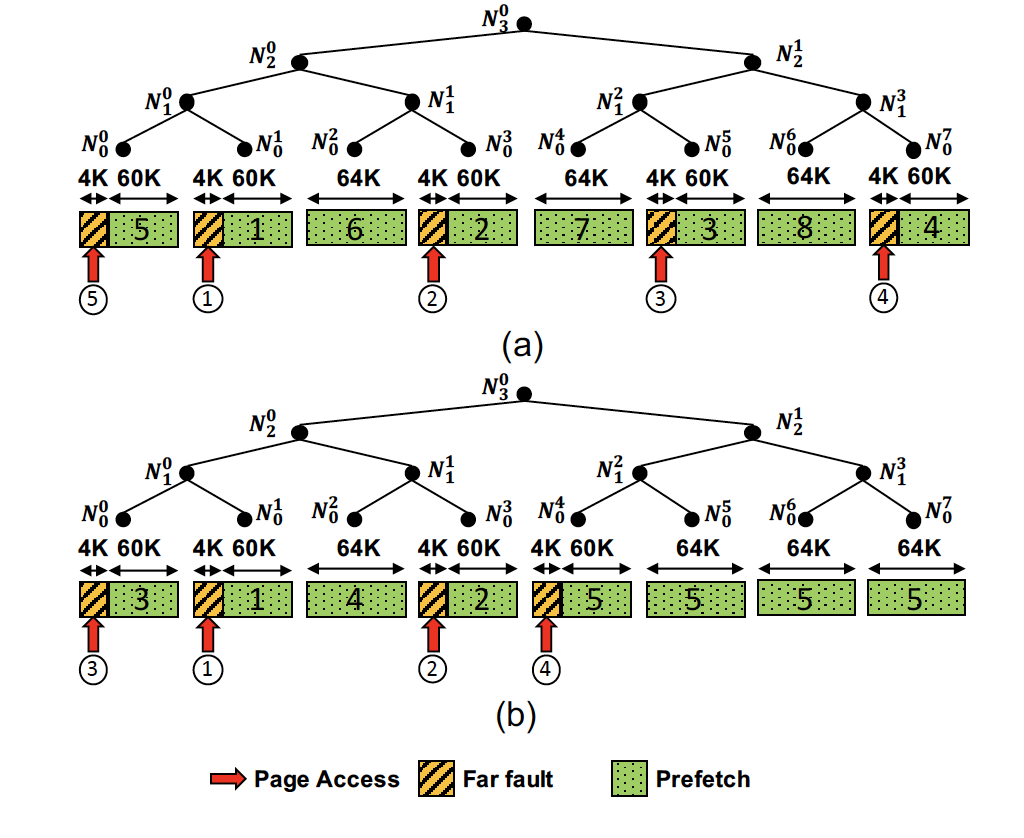
\includegraphics[width=.90\textwidth,keepaspectratio]{figures1/prefetchers.elf}
      \captionsetup{width=.90\textwidth}
      \caption{Demonstration ofTBNp on 512 KB memory chunk for two different page access patterns.}
      \label{fig:prefetchers}
    \end{figure}

The semantics of TBNp demands that every cudaMallocManaged allocation is first logically divided into 2MB large pages. Then, these 2MB large pages are further divided into logical 64KB basic blocks to create a full binary tree  per large page boundary. By the definition of a full binary tree, every node has exactly 2 children nodes. The root node of each binary tree corresponds to the virtual address of a 2MB large page and the leaf-level nodes correspond to the virtual addresses of the 64KB basic blocks. If the user-specified size of an allocation is not a perfect multiple of 2MB, then the remainder allocation is rounded up to the next $2^i * 64$KB and another full binary tree is created.

The maximum memory capacity of a node in the full binary tree can be calculated as $2^h * 64$KB, where h is the height of a node and h = 0 at the leaf level. On every far-fault, the GMMU first identifies the 64KB basic block corresponding to the faulty page being requested. With the understanding that upon migrating, 16 pages in the basic block will be validated in the GPU page table, GMMU then recalculates the to-be valid size of its parent and grandparent up to the root node of the tree. Here and henceforth, valid size is the size of all valid pages corresponding to the leaf-nodes belonging to a given node. At any point, if GMMU discovers the to-be valid size of a node is strictly greater than 50\% of the maximum memory capacity at this level, it tries to balance the valid sizes between the two children of that node. This balancing process is recursively pushed down to the children which have not reached the maximum valid size quota. This balancing act identifies basic blocks for prefetching. This process continues till no more basic blocks at leaf level can be identified as prefetch candidates and the to-be valid size of any non-leaf node including root is not more than 50\% of maximum size capacity at its level. 

In Figure \ref{fig:prefetchers}, Tree-based Neighborhood Prefetcher is demonstrated by two examples. Both of these examples explain the semantics on 512KB memory chunk for simplicity. These examples use $N_h^I$ to denote a node in the full binary tree, where $h$ is the height of the node and i is the numeric position of the node in that particular level. These examples assume initially all pages in this 512KB allocation are invalid with valid bit not set in the GPU’s page table and thus every first access to a page causes a far-fault. In the first example, for the first four far-faults, GMMU identifies the corresponding basic blocks $N^1_0$ , $N^3_0$ , $N^5_0$ , and $N^7_0$ for migration. As the first byte of every basic block is accessed, the basic blocks are split into 4KB page-fault groups and 60KB prefetch groups. All memory transfers are serialized in time. After these first four accesses, each of nodes $N^1_0$ , $N^3_0$ , $N^5_0$ , and $N^7_0$ has 64KB valid pages. Then, GMMU traverses the full tree to update the valid page size for all the parent nodes and thus each node at $h = 1$ ($N^1_0$ , $N^1_1$ , $N^2_1$ , and $N^3_1$) has 64KB valid pages. When the fifth access occurs, GMMU discovers that $N^0_1$ and $N^0_2$ will have 128KB and 192KB valid pages respectively. For $N^0_2$, the to-be valid size is greater than 50\% of the maximum valid size of 256KB. Hence, the right child $N^1_1$ is identified for prefetching. This decision is then pushed down to the children. This process identifies the basic block $N^2_0$ as a prefetch candidate. Further, GMMU discovers that after prefetching $N^2_0$, $N^0_3$ will have 320KB of valid pages which is more than 50\% of the maximum valid size of 512KB. Then, node $N^0_3$ pushes prefetch request to the node $N^1_2$ which in turn pushes it to its children. This process identifies basic blocks $N^4_0$ and $N^6_0$ for further prefetching.

In the second example, the first two far-faults cause migration of basic blocks $N^1_0$ and $N^3_0$. GMMU traverses the tree to update the valid size of nodes $N^0_1$ and $N^1_1$ as 64KB each. At the third far-fault, as basic block $N^0_0$ is migrated, the estimated valid sizes for nodes $N^0_1$, and $N^0_2$ are updated as 128KB and 192KB respectively. As the valid size of $N^0_2$ is more than 50\% of the maximum valid size of 256KB, $N^2_0$ is identified for prefetching. After this point, the $N^0_2$ is fully balanced and both $N^0_2$ and $N^0_3$ have exactly 256KB of valid pages. On fourth access, GMMU discovers that the valid size of $N^0_3$ will be 320KB which is more than 50\% of the maximum memory size it can hold. This imbalance causes prefetching of nodes $N^5_0$ , $N^6_0$, and $N^7_0$. Note at this point as GMMU finds four consecutive basic blocks, it groups them together to take advantage of higher bandwidth. Then, based on the page fault, it splits this 256KB into two transfers: 4KB and 252KB. An interesting point to observe here is that for a full binary tree of 2MB size, TBNp can prefetch at most 1020KB at once in a scenario similar to the second example.